% !TeX root = RJwrapper.tex
\title{Variable Importance Plots: An Introduction to the \pkg{vip} Package}
\author{by Brandon M. Greenwell and Bradley C. Boehmke}

\maketitle

\abstract{
In the era of "big data", it is becoming more of a challenge to not only build state-of-the-art predictive models, but also gain an understanding of what's really going on in the data. For example, it is often of interest to know which, if any, of the predictors in a fitted model are relatively influential on the predicted outcome. Some modern algorithms---like random forests (RFs) and gradient boosted decision trees (GBMs)---have a natural way of quantifying the importance or relative influence of each feature. Other algorithms---like naive Bayes classifiers and support vector machines---are not capable of doing so and \dfn{model-agnostic approaches} are generally used to measure each predictor’s importance. Enter \pkg{vip}, an R package for constructing variable importance scores/plots for many types of supervised learning algorithms using model-specific and novel model-agnostic approaches. We'll also discuss a novel way to display both feature importance and feature effects together using \dfn{sparklines}, a very small line chart conveying the general shape or variation in some feature that can be directly embedded in text or tables.
}


% ------------------------------------------------------------------------------
\section{Introduction}
% ------------------------------------------------------------------------------

Too often machine learning (ML) models are summarized using a single metric (e.g., cross-validated accuracy) and then put into production. Although we often care about the predictions from these models, it is becoming routine to also understand the predictions! Understanding how an ML model makes its predictions helps build trust in the model and is the fundamental idea of the emerging field of \dfn{interpretable machine learning} (IML). For an in-depth discussion on IML, see \citet{molnar-2019-iml}. In this paper, we focus on global methods for quantifying the importance of features in an ML model. Computing variable importance (VI) and communicating them through variable importance plots (VIPs) is a fundamental component of IML and is the main topic of this paper.

VI scores and VIPs can be constructed for general ML models using a number of packages. The \CRANpkg{iml} package \citep{iml-pkg} provides the \code{FeatureImp()} function which computes feature importance for general prediction models using the permutation approach (discussed later). It is written in \CRANpkg{R6} \citep{R6-pkg} and allows the user to specify a generic loss function or select one from a pre-defined list (e.g., \code{loss = "mse"} for mean squared error). It also allows the user to specify whether importance is measured as the difference or as the ratio of the original model error and the model error after permutation. The user can also specify the number of repetitions used when permuting each feature to help stabilize the variability in the procedure.

The \CRANpkg{ingredients} package \citep{ingredients-pkg} also provides permutation-based VI scores through the \code{feature\_importance()} function. (Note that this function recently replaced the now deprecated \CRANpkg{DALEX} function \code{variable\_importance()} \citep{DALEX-pkg}.) Similar to \code{iml::FeatureImp()}, this function allows the user to specify a loss function and how the importance scores are computed (e.g., using the difference or ratio). It also provides an option to sample the training data before shuffling the data to compute importance (the default is to use \code{n\_sample = 1000}). This can help speed up computation.

The \CRANpkg{caret} package \citep{caret-pkg} includes a general \code{varImp()} function for computing model-specific and filter-based VI scores. Filter-based approaches, which are described in \citet{applied-kuhn-2013}, do not make use of the fitted model to measure VI. They also do not take into account the other predictors in the model. For regression problems, a popular filter-based approach to measuring the VI of a numeric predictor $x$ is to first fit a flexible nonparametric model between $x$ and the target $Y$; for example, the locally-weighted polynomial regression (LOWESS) method developed by \citet{robust-cleveland-1979}. From this fit, a pseudo-$R^2$ measure can be obtained from the resulting residuals and used as a measure of VI. For categorical predictors, a different method based on standard statistical tests (e.g., $t$-tests and ANOVAs) can be employed; see \citet{applied-kuhn-2013} for details. For classification problems, an area under the ROC curve (AUC) statistic can be used to quantify predictor importance. The AUC statistic is computed by using the predictor $x$ as input to the ROC curve. If $x$ can reasonably separate the classes of $Y$, that is a clear indicator that $x$ is an important predictor (in terms of class separation) and this is captured in the corresponding AUC statistic. For problems with more than two classes, extensions of the ROC curve or a one-vs-all approach can be used.

If you use the \CRANpkg{mlr} interface for fitting ML models \citep{mlr-pkg}, then you can use the \code{getFeatureImportance()} function to extract model-specific VI scores from various tree-based models (e.g., RFs and GBMs). Unlike \pkg{caret}, the model needs to be fit via the \pkg{mlr} interface; for instance, you cannot use \code{getFeatureImportance()} on a \CRANpkg{gbm} model \citep{gbm-pkg} unless it was fit using \pkg{mlr}.

While the \pkg{iml} and \pkg{DALEX} packages provide model-agnostic approaches to computing VI, \pkg{caret}, and to some extent \pkg{mlr}, provide model-specific approaches (e.g., using the absolute value of the $t$-statistic for linear models) as well less accurate filter-based approaches . Furthermore, each package has a completely different interface (e.g., \pkg{iml} is written in R6). The \CRANpkg{vip} package \citep{vip-pkg} strives to provide a consistent interface to both model-specific and model-agnostic approaches to feature importance that is simple to use. The three most important functions exported by \pkg{vip} are described below:

\begin{itemize}
 
  \item \code{vi()} computes VI scores using model-specific or model-agnostic approaches (the results are always returned as a tibble \citep{tibble-pkg});
  
  \item \code{vip()} constructs VIPs using model-specific or model-agnostic approaches with \CRANpkg{ggplot2}-style graphics \citep{ggplot2-pkg};
  
  \item \code{add\_sparklines()} adds a novel sparkline representation of feature effects (e.g., \dfn{partial dependence plots}) to any VI table produced by \code{vi()}.

\end{itemize}

There's also a function called \code{vint()} (for variable interactions) but is experimental and will not be discussed here; the interested reader is pointed to \citet{greenwell-simple-2018}. Note that \code{vi()} is actually a wrapper around four workhorse functions, \code{vi\_model()}, \code{vi\_ice()}, \code{vi\_pdp()}, and \code{vi\_permute()}, that compute various types of VI scores. The first computes model-specific VI scores, while the latter three produce model-agnostic ones. The workhorse function that actually gets called is controlled by the \code{method} argument in \code{vi()}; the default is \code{method = "model"} which corresponds to model-specific VI (see \code{?vip::vi} for details and links to further documentation). 


% ------------------------------------------------------------------------------
\section{Constructing VIPs in R}
% ------------------------------------------------------------------------------

We'll illustrate major concepts using the Friedman 1 benchmark problem described in \citet{multivariate-friedman-1991} and \citet{bagging-breiman-1996}: 

\begin{equation}
  Y_i = 10 \sin\left(\pi X_{1i} X_{2i}\right) + 20 \left(X_{3i} - 0.5\right) ^ 2 + 10 X_{4i} + 5 X_{5i} + \epsilon_i, \quad i = 1, 2, \dots, n,
\label{eqn:friedman1}
\end{equation}

where $\epsilon_i \stackrel{iid}{\sim} N\left(0, \sigma^2\right)$. Data from this model can be generated using the \code{mlbench.friedman1()} function available in the \CRANpkg{mlbench} package \citep{mlbench-pkg}. The features consist of 10 independent variables uniformly distributed on the interval $\left[0,1\right]$; however, only 5 out of these 10 are actually used in the true model. The code chunk below simulates 500 observations from the model in Equation~\eqref{eqn:friedman1} with $\sigma = 1$ (the default); see \code{mlbench::mlbench.friedman1} for details.

\begin{example}
# Simulate training data
set.seed(101)  # for reproducibility
trn <- as.data.frame(mlbench::mlbench.friedman1(500))  # ?mlbench.friedman1
names(trn) <- gsub("^x\\.", replacement = "X", x = names(trn))  # to match notation

# Inspect data
tibble::as_tibble(trn)
#> Warning: `as.tibble()` is deprecated, use `as_tibble()` (but mind the new semantics).
#> This warning is displayed once per session.
#> # A tibble: 500 x 11
#>        X1    X2    X3    X4     X5      X6    X7    X8    X9   X10     y
#>     <dbl> <dbl> <dbl> <dbl>  <dbl>   <dbl> <dbl> <dbl> <dbl> <dbl> <dbl>
#>  1 0.372  0.406 0.102 0.322 0.693  0.758   0.518 0.530 0.878 0.763 14.9 
#>  2 0.0438 0.602 0.602 0.999 0.776  0.533   0.509 0.487 0.118 0.176 15.3 
#>  3 0.710  0.362 0.254 0.548 0.0180 0.765   0.715 0.844 0.334 0.118 15.1 
#>  4 0.658  0.291 0.542 0.327 0.230  0.301   0.177 0.346 0.474 0.283 10.7 
#>  5 0.250  0.794 0.383 0.947 0.462  0.00487 0.270 0.114 0.489 0.311 17.6 
#>  6 0.300  0.701 0.992 0.386 0.666  0.198   0.924 0.775 0.736 0.974 18.3 
#>  7 0.585  0.365 0.283 0.488 0.845  0.466   0.715 0.202 0.905 0.640 14.6 
#>  8 0.333  0.552 0.858 0.509 0.697  0.388   0.260 0.355 0.517 0.165 17.0 
#>  9 0.622  0.118 0.490 0.390 0.468  0.360   0.572 0.891 0.682 0.717  8.54
#> 10 0.546  0.150 0.476 0.706 0.829  0.373   0.192 0.873 0.456 0.694 15.0 
#> # … with 490 more rows
\end{example}

From Equation~\eqref{eqn:friedman1}, it should be clear that features $X_1$--$X_5$ are the most important! (The others don't influence $Y$ at all.) Also, based on the form of the model, we'd expect $X_4$ to be the most important feature, probably followed by $X_1$ and $X_2$ (both comparably important), with $X_5$ probably less important. The influence of $X_3$ is harder to determine due to its quadratic nature, but it seems likely that this nonlinearity will suppress the variable's influence over its observed range (i.e., 0--1).


% ------------------------------------------------------------------------------
\section{Model-specific VI}
% ------------------------------------------------------------------------------

Some machine learning algorithms have their own way of quantifying the importance of each feature. We describe some of these in the subsections that follow. The issue with model-specific VI scores is that they are not necessarily comparable across different types of models. For example, directly comparing the impurity-based VI scores from tree-based models to the $t$-statistic from linear models.

\subsection{Decision trees and tree ensembles}

Decision trees probably offer the most natural model-specific approach to quantifying the importance of each feature. In a binary decision tree, at each node $t$, a single predictor is used to partition the data into two homogeneous groups. The chosen predictor is the one that maximizes some measure of improvement $i^t$. The relative importance of predictor $X$ is the sum of the squared improvements over all internal nodes of the tree for which $X$ was chosen as the partitioning variable; see \citet{classification-breiman-1984} for details. This idea also extends to ensembles of decision trees, such as RFs and GBMs. In ensembles, the improvement score for each predictor is averaged across all the trees in the ensemble. Fortunately, due to the stabilizing effect of averaging, the improvement-based VI metric is often more reliable in large ensembles; see \citet[p. 368]{hastie-elements-2009}. RFs offer an additional method for computing VI scores. The idea is to use the leftover out-of-bag (OOB) data to construct validation-set errors for each tree. Then, each predictor is randomly shuffled in the OOB data and the error is computed again. The idea is that if variable $X$ is important, then the validation error will go up when $X$ is perturbed in the OOB data. The difference in the two errors is recorded for the OOB data then averaged across all trees in the forest. Later on, we'll discuss a more general permutation method that can be applied to any supervised learning model.

To illustrate, we fit a CART-like regression tree, RF, and GBM to the simulated training data. (Note: there are a number of different packages available for fitting these types of models, we just picked popular implementations for illustration.)

\begin{example}
# Load required packages
library(rpart)          # for fitting CART-like decision trees
library(randomForest)   # for fitting RFs
library(xgboost)        # for fitting GBMs

# Fit a single regression tree
tree <- rpart(y ~ ., data = trn)

# Fit an RF
set.seed(101)
rfo <- randomForest(y ~ ., data = trn, importance = TRUE)

# Fit a GBM
set.seed(102)
bst <- xgboost(
  data = data.matrix(subset(trn, select = -y)),
  label = trn$y, 
  objective = "reg:linear",
  nrounds = 100, 
  max_depth = 5, 
  eta = 0.3,
  verbose = 0  # suppress printing
)
\end{example}

Each of the above packages include the ability to compute VI scores for all the features in the model; however, the implementation is rather package specific, as shown in the code chunk below. The results are displayed in Figure~\ref{fig:vi-plots} (the code to reproduce these plots has been omitted but can be made available upon request).

\begin{example}
# Extract VI scores from each model
vi_tree <- tree$variable.importance
vi_rfo <- rfo$variable.importance
vi_bst <- xgb.importance(model = bst)
\end{example}

\begin{figure}[!htb]
  \centering 
  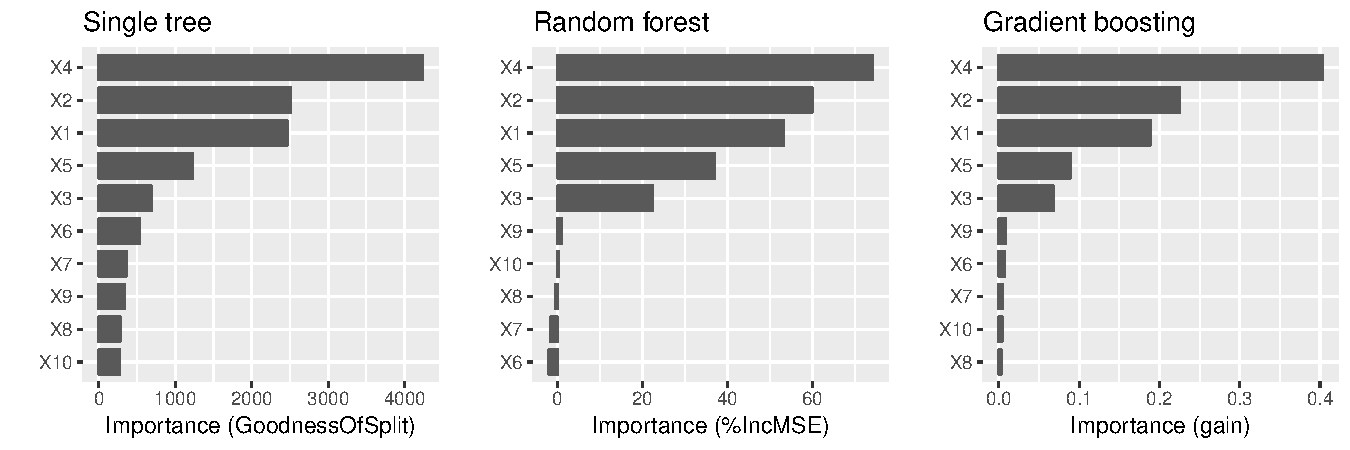
\includegraphics[width=1\linewidth]{figures/vi-plots} 
  \caption{model-specific VIPs for the three different tree-based models fit to the simulated Friedman data.}
  \label{fig:vi-plots}
\end{figure}

As we would expect, all three methods rank the variables \code{X1}--\code{X5} as more important than the others. While this is good news, it is unfortunate that we have to remember the different functions and ways of extracting and plotting VI scores from various model fitting functions. This is one place where \pkg{vip} can help...one function to rule them all! Once \pkg{vip} is loaded, we can use \code{vi()} to extract a tibble of VI scores.

\begin{example}
# Load required packages
library(vip)

# Compute model-specific VI scores
vi(tree)  # CART-like decision tree
#> # A tibble: 10 x 2
#>    Variable Importance
#>    <chr>         <dbl>
#>  1 X4            4234.
#>  2 X2            2513.
#>  3 X1            2461.
#>  4 X5            1230.
#>  5 X3             688.
#>  6 X6             533.
#>  7 X7             357.
#>  8 X9             331.
#>  9 X8             276.
#> 10 X10            275.

vi(rfo)   # RF
#> # A tibble: 10 x 2
#>    Variable Importance
#>    <chr>         <dbl>
#>  1 X4           74.2  
#>  2 X2           59.9  
#>  3 X1           53.3  
#>  4 X5           37.1  
#>  5 X3           22.5  
#>  6 X9            1.05 
#>  7 X10           0.254
#>  8 X8           -0.408
#>  9 X7           -1.56 
#> 10 X6           -2.00

vi(bst)   # GBM
#> # A tibble: 10 x 2
#>    Variable Importance
#>    <chr>         <dbl>
#>  1 X4          0.403  
#>  2 X2          0.225  
#>  3 X1          0.189  
#>  4 X5          0.0894 
#>  5 X3          0.0682 
#>  6 X9          0.00802
#>  7 X6          0.00746
#>  8 X7          0.00400
#>  9 X10         0.00377
#> 10 X8          0.00262
\end{example}

Notice how the \code{vi()} function always returns a tibble\footnote{Technically, it's a tibble with an additional \code{"vi"} class.} with two columns: \code{Variable} and \code{Importance} (the exceptions are coefficient-based models which also include a \code{Sign} column giving the sign of the corresponding coefficient and permutation importance involving multiple Monte Carlo simulations, but more on that later). Also, by default, \code{vi()} always orders the VI scores from highest to lowest; this, among other options, can be controlled by the user (see \code{?vip::vi} for details). Plotting VI scores with \code{vip()} is just as straightforward. For example, the following code can be used to reproduce Figure~\ref{fig:vi-plots}.

\begin{example}
p1 <- vip(tree) + ggtitle("Single tree")
p2 <- vip(rfo) + ggtitle("Random forest")
p3 <- vip(bst) + ggtitle("Gradient boosting")

# Figure 1
grid.arrange(p1, p2, p3, nrow = 1)
\end{example}

Notice how the \code{vip()} function always returns a \code{"ggplot"} object (by default, this will be a bar plot). For large models with many features, a dot plot is more effective (in fact, a number of useful plotting options can be fiddled with). Below we call \code{vip()} and change a few useful options (the resulting plot is displayed in Figure~\ref{fig:dot-plot}). Note that we can also call \code{vip()} directly on a \code{"vi"} objects if it's already been constructed.

\begin{example}
# Load required packages
library(ggplot2)  # for theme_light() function

vip(bst, num_features = 5, bar = FALSE, color, horizontal = FALSE, 
    color = "red", shape = 17, size = 4) +
  theme_light()
\end{example}

\begin{figure}[!htb]
  \centering 
  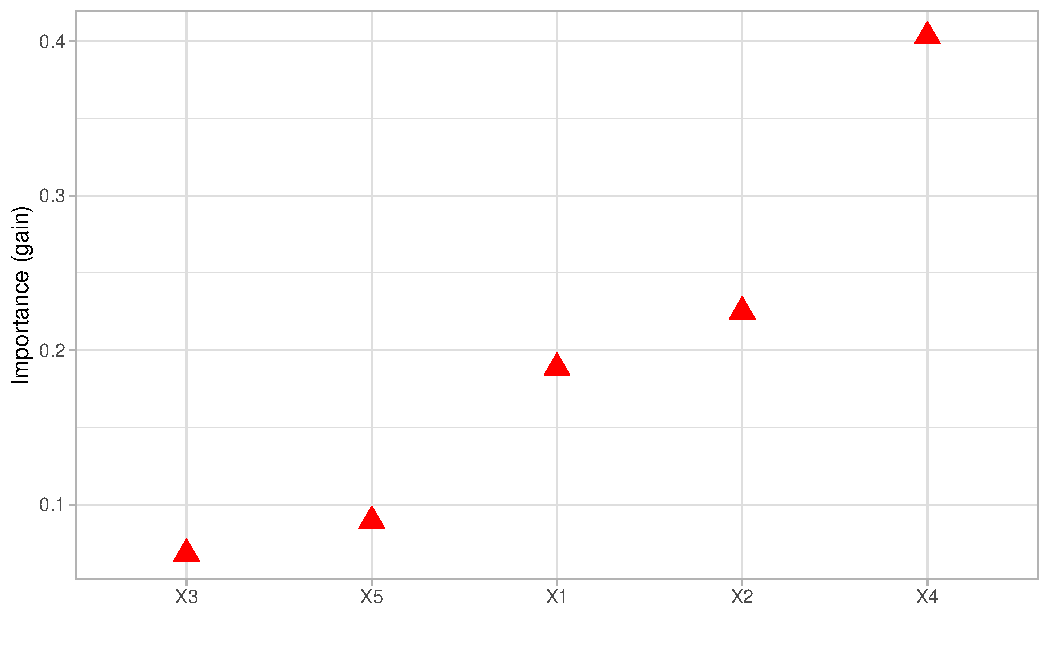
\includegraphics[width=1\linewidth]{figures/dot-plot} 
  \caption{Illustrating various options available in \code{vip()}.}
  \label{fig:dot-plot}
\end{figure}


\subsection{Linear models}

In multiple linear regression, or linear models (LMs), the absolute value of the $t$-statistic (or some other scaled variant of the estimated coefficients) is commonly used as a measure of VI. The same idea also extends to generalized linear models (GLMs). In the code chunk below, we fit an LM to the simulated \code{trn} data set allowing for all main effects and two-way interactions, then use the \code{step()} function to perform backward elimination. The resulting VIP is displayed in Figure~\ref{fig:vip-step}.

\begin{example}
# Fit a LM
linmod <- lm(y ~ .^2, data = trn)
backward <- step(linmod, direction = "backward", trace = 0)

# Extract VI scores
(vi_backward <- vi(backward))
#> # A tibble: 21 x 3
#>    Variable Importance Sign 
#>    <chr>         <dbl> <chr>
#>  1 X4            14.2  POS  
#>  2 X2             7.31 POS  
#>  3 X1             5.63 POS  
#>  4 X5             5.21 POS  
#>  5 X3:X5          2.46 POS  
#>  6 X1:X10         2.41 NEG  
#>  7 X2:X6          2.41 NEG  
#>  8 X1:X5          2.37 NEG  
#>  9 X10            2.21 POS  
#> 10 X3:X4          2.01 NEG  
#> # … with 11 more rows

# Plot VI scores; by default, `vip()` displays the top ten features
vip(vi_backward, num_features = length(coef(backward)), 
    bar = FALSE, horizontal = FALSE)
\end{example}

\begin{figure}[!htb]
  \centering 
  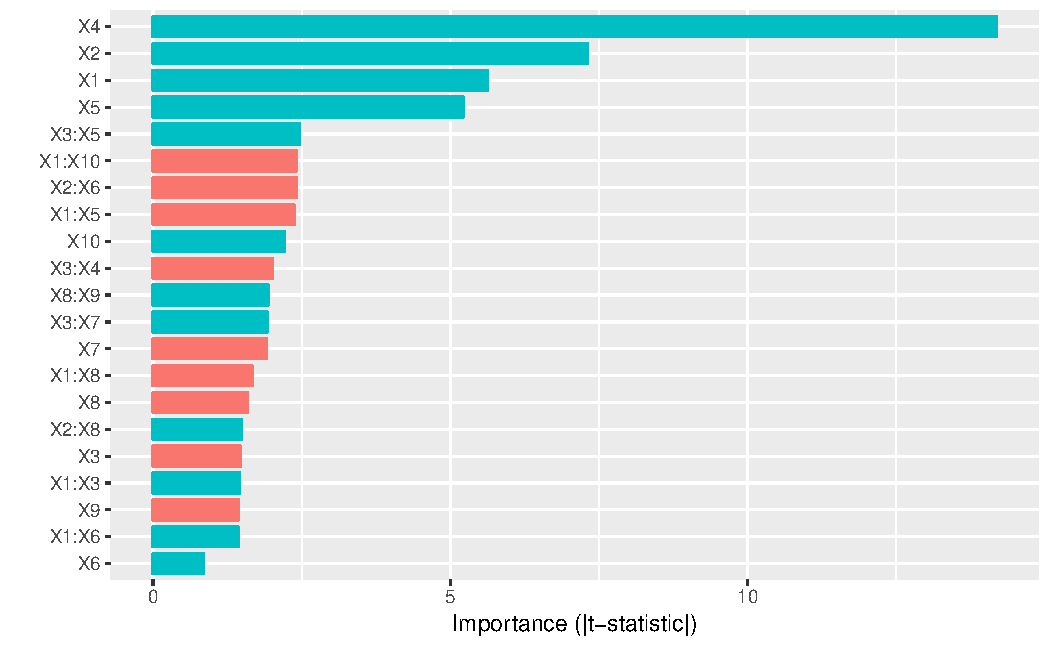
\includegraphics[width=1\linewidth]{figures/vip-step} 
  \caption{Example VIP from a linear model fit to the simulated Friedman data.}
  \label{fig:vip-step}
\end{figure}

One issue with computing VI scores for LMs using the $t$-statistic approach is that a score is assigned to each term in the model, rather than to each individual feature! We can solve this problem using one of the model-agnostic approaches discussed later.

Multivariate adaptive regression splines (MARS), which were introduced in \citet{multivariate-friedman-1991}, is an automatic regression technique and can be seen as a generalization of LMs and GLMs. In the MARS algorithm, the contribution (or VI score) for each predictor is determined using a generalized cross-validation (GCV) statistic (though, other statistics can also be used; see \code{?vip::vi\_model} for details). An example using the \CRANpkg{earth} package \citep{earth-pkg} is given below (the results are plotted in Figure~\ref{fig:vip-earth}):

\begin{example}
# Load required packages
library(earth)

# Fit a MARS model
mars <- earth(y ~ ., data = trn, degree = 2, pmethod = "exhaustive")

# Extract VI scores
vi(mars, type = "gcv")
#> # A tibble: 10 x 2
#>    Variable Importance
#>    <chr>         <dbl>
#>  1 X4            100  
#>  2 X1             83.2
#>  3 X2             83.2
#>  4 X5             59.3
#>  5 X3             43.5
#>  6 X6              0  
#>  7 X7              0  
#>  8 X8              0  
#>  9 X9              0  
#> 10 X10             0

# Plot VI scores
vip(mars)
\end{example}

\begin{figure}[!htb]
  \centering 
  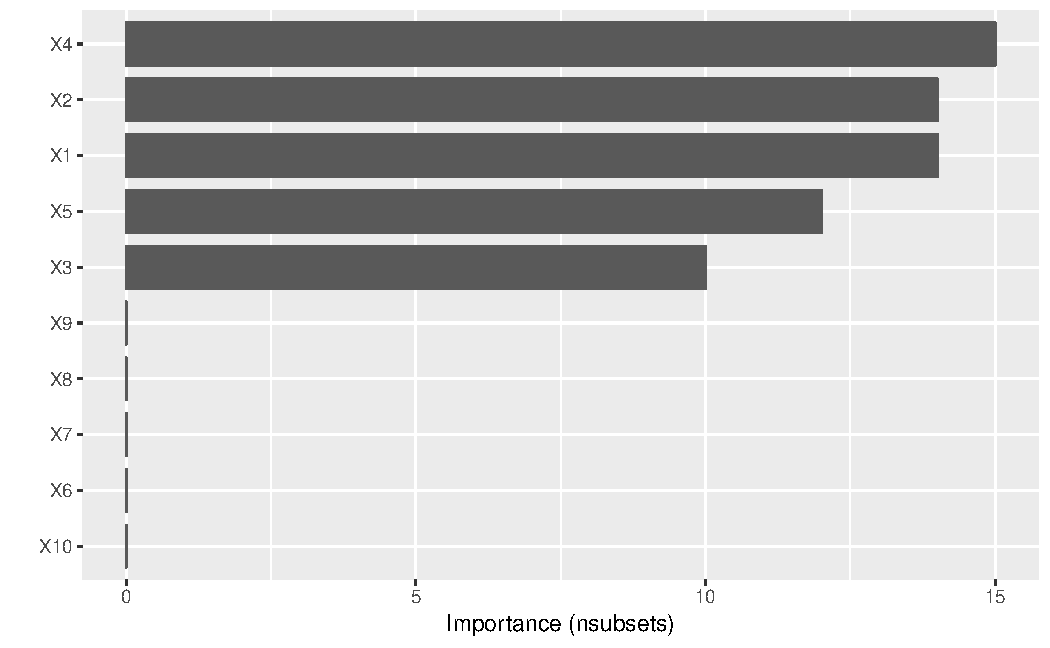
\includegraphics[width=1\linewidth]{figures/vip-earth} 
  \caption{Example VIP from a MARS model fit to the simulated Friedman data.}
  \label{fig:vip-earth}
\end{figure}

To access VI scores directly in \pkg{earth}, you can use the \code{earth::evimp()} function.

\subsection{Neural networks}

For neural netwroks (NNs), two popular methods for constructing VI scores are the Garson algorithm \citep{interpreting-garson-1991}, later modified by \citet{back-goh-1995}, and the Olden algorithm \citep{accurate-olden-2004}. For both algorithms, the basis of these VI scores is the network’s connection weights. The Garson algorithm determines VI by identifying all weighted connections between the nodes of interest. Olden’s algorithm, on the other hand, uses the products of the raw connection weights between each input and output neuron and sums these products across all hidden neurons. This has been shown to outperform the Garson method in various simulations. For DNNs, a similar method due to \citet{data-gedeon-1997} considers the weights connecting the input features to the first two hidden layers (for simplicity and speed); but this method can be slow for large networks. We illustrate these two methods below using \code{vip()} with the \CRANpkg{nnet} package \citep{nnet-pkg} (see the results in Figure~\ref{fig:vip-earth}).

\begin{example}
# Load required packages
library(nnet)

# Fit a neural network
set.seed(0803)
nn <- nnet(y ~ ., data = trn, size = 7, decay = 0.1, linout = TRUE)

# VIPs
p1 <- vip(nn, type = "garson")
p2 <- vip(nn, type = "olden")

# Figure 5
grid.arrange(p1, p2, nrow = 1)
\end{example}

\begin{figure}[!htb]
  \centering 
  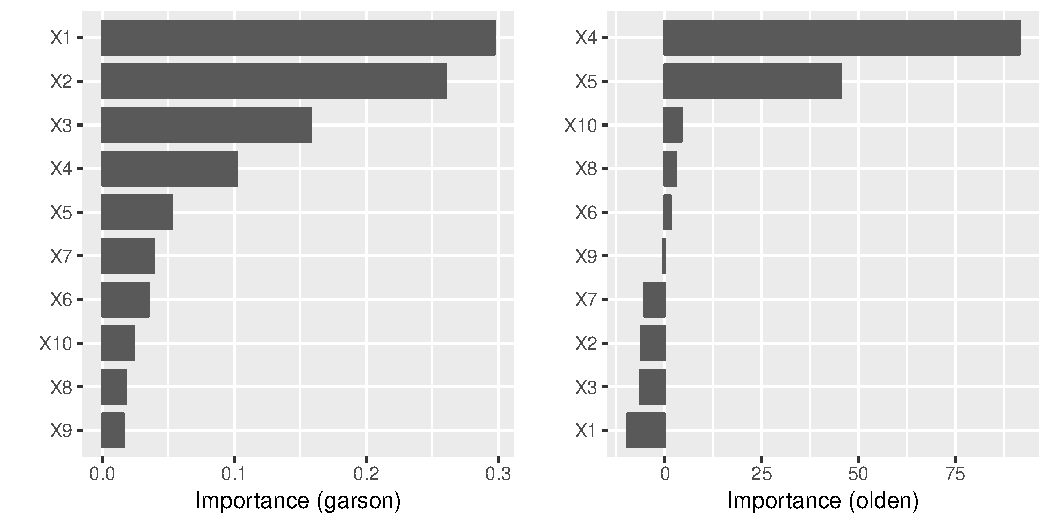
\includegraphics[width=1\linewidth]{figures/vip-model-nn} 
  \caption{Example VIPs from a single-hidden-layer NN fit to the simulated Friedman data.}
  \label{fig:vip-earth}
\end{figure}


% ------------------------------------------------------------------------------
\section{Model-agnostic VI}
% ------------------------------------------------------------------------------

Model-agnostic interpredibility separates interpretation from the model. Compared to model-specific approaches, model-agnostic VI methods are more flexible and can be applied to any supervised learning algorithm. In this section, we discuss model-agnostic methods for quantifying global feature importance using three different approaches: 1) partial dependence plots (PDPs), 2) \dfn{individual conditional expectation} (ICE) curves, and 3) permutation-based feature importance. For specific details on approaches 1)--2), see \citet{greenwell-simple-2018}.


\subsection{PDP method}

Our first model-agnostic approach is based on quantifying the "flatness" of the PDPs of each feature. PDPs help visualize the effect of low cardinality subsets of the feature space on the estimated prediction surface (e.g., main effects and two/three-way interaction effects.). PDPs provide model-agnostic interpretations and can be constructed in the same way for any supervised learning algorithm; for an overview, see \citet{greenwell-pdp-2017}. Below, we fit a projection pursuit regression (PPR) model and construct PDPs for each feature using the \CRANpkg{pdp} package \citet{greenwell-pdp-2017}. The results are displayed in Figure~\ref{fig:pdp-ppr}. Notice how the PDPs for the uninformative features are relatively flat compared to the PDPs for features \code{X1}--\code{X2}!

\begin{example}
# Load required packages
library(pdp)

# Fit a PPR model (nterms was chosen using the caret package with 5 repeats of 
# 5-fold cross-validation)
pp <- ppr(y ~ ., data = trn, nterms = 11)  

# PDPs for all 10 features
features <- paste0("X", 1:10)
pdps <- lapply(features, FUN = function(feature) {
  pd <- partial(pp, pred.var = feature)
  autoplot(pd) + 
    ylim(range(trn$y)) + 
    theme_light()
})
grid.arrange(grobs = pdps, ncol = 5)
\end{example}

\begin{figure}[!htb]
  \centering 
  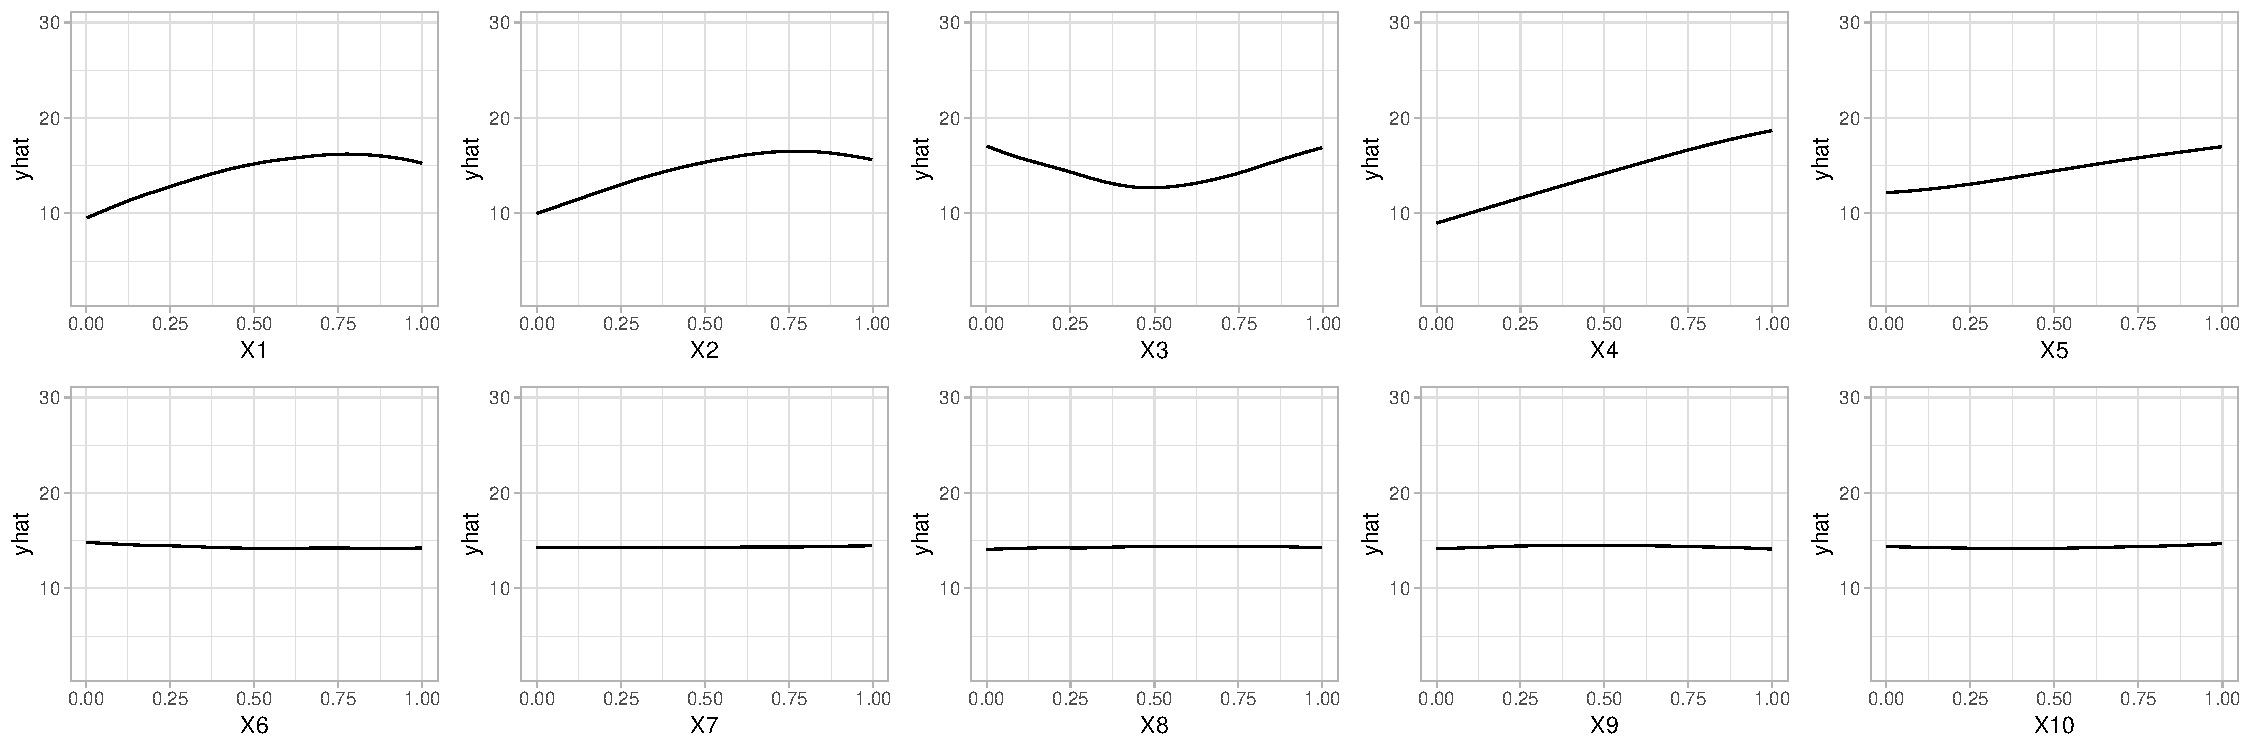
\includegraphics[width=1\linewidth]{figures/pdp-ppr} 
  \caption{PDPs of main effects in the PPR model fit to the simulated Friedman data.}
  \label{fig:pdp-ppr}
\end{figure}

Next, we compute PDP-based VI scores for the PPR and NN models. The PDP method constructs VI scores that quantify the relative "flatness" of each PDP (by default, this is defined by computing the standard deviation of the $y$-axis values for each PDP). To use the PDP method, specify \code{method = "pdp"} in the call to \code{vi()} or \code{vip()}:

\begin{example}
# Fit a PPR model (nterms was chosen using the caret package with 5 repeats of 
# 5-fold cross-validation)
pp <- ppr(y ~ ., data = trn, nterms = 11)  

# Plot VI scores
p1 <- vip(pp, method = "pdp") + ggtitle("PPR")
p2 <- vip(nn, method = "pdp") + ggtitle("NN")

# Figure 7
grid.arrange(p1, p2, ncol = 2)
\end{example}

In Figure~\ref{fig:pdp-ppr-nn} we display the PDP-based feature importance for the previously obtained PPR and NN models. These VI scores essentially capture the variability in the partial dependence values for each main effect.

\begin{figure}[!htb]
  \centering 
  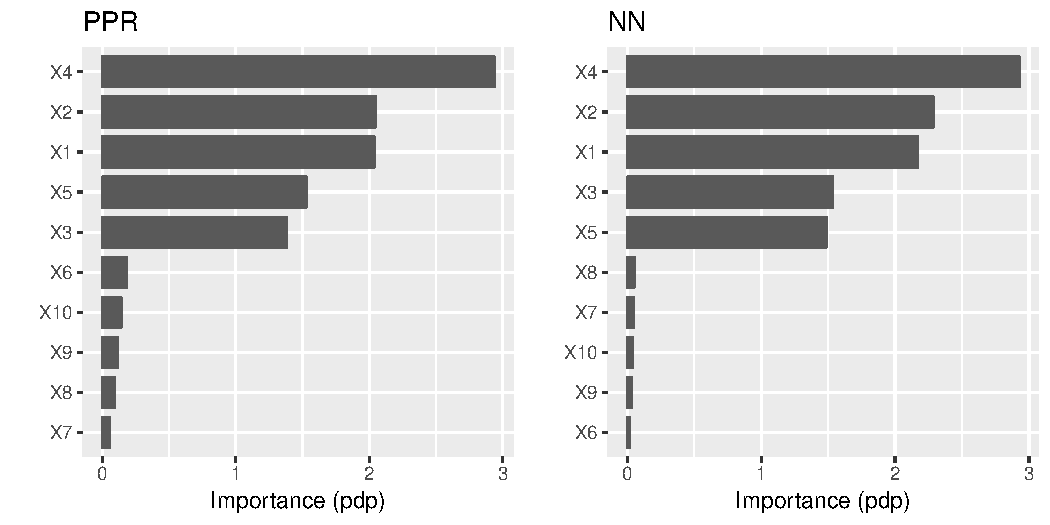
\includegraphics[width=1\linewidth]{figures/vip-ppr-nn} 
  \caption{PDP-based feature importance for the PPR and NN models fit to the simulated Friedman data.}
  \label{fig:pdp-ppr-nn}
\end{figure}


\subsection{ICE curve method}

The ICE curve method is similar to the PDP method. The only difference is that we measure the "flatness" of each ICE curve and then aggregate the results (e.g., by averaging). If there are no (substantial) interaction effects, using \code{method = "ice"} will produce results similar to using \code{method = "pdp"}. However, if strong interaction effects are present, they can obfuscate the main effects and render the PDP-based approach less useful (since the PDPs for important features can be relatively flat when certain interactions are present; see \citet{goldstein-peeking-2015} for details). In fact, it is probably safest to always use \code{method = "ice"}.

Below, we display the ICE curves for each feature in the PPR model using the same $y$-axis scale; see Figure~\ref{fig:ice-ppr}. Again, there is a clear difference between the ICE curves for features \code{X1}--\code{X5} and \code{X6}--\code{X10}; the later being relatively flat by comparison. Also, notice how the ICE curves within each feature are relatively parallel (if the ICE curves within each feature were perfectly parallel, the standard deviation for each curve would be the same and the results will be identical to the PDP method). In this example, the interaction term between \code{X1} and \code{X2} does not obfuscate the PDPs for the main effects and the results are not much different.

\begin{example}
# ICE curves for all 10 features
ice_curves <- lapply(features, FUN = function(feature) {
  ice <- partial(pp, pred.var = feature, ice = TRUE)
  autoplot(ice, alpha = 0.1) + 
    ylim(range(trn$y)) +
    theme_light()
})

# Figure 8
grid.arrange(grobs = ice_curves, ncol = 5)
\end{example}

\begin{figure}[!htb]
  \centering 
  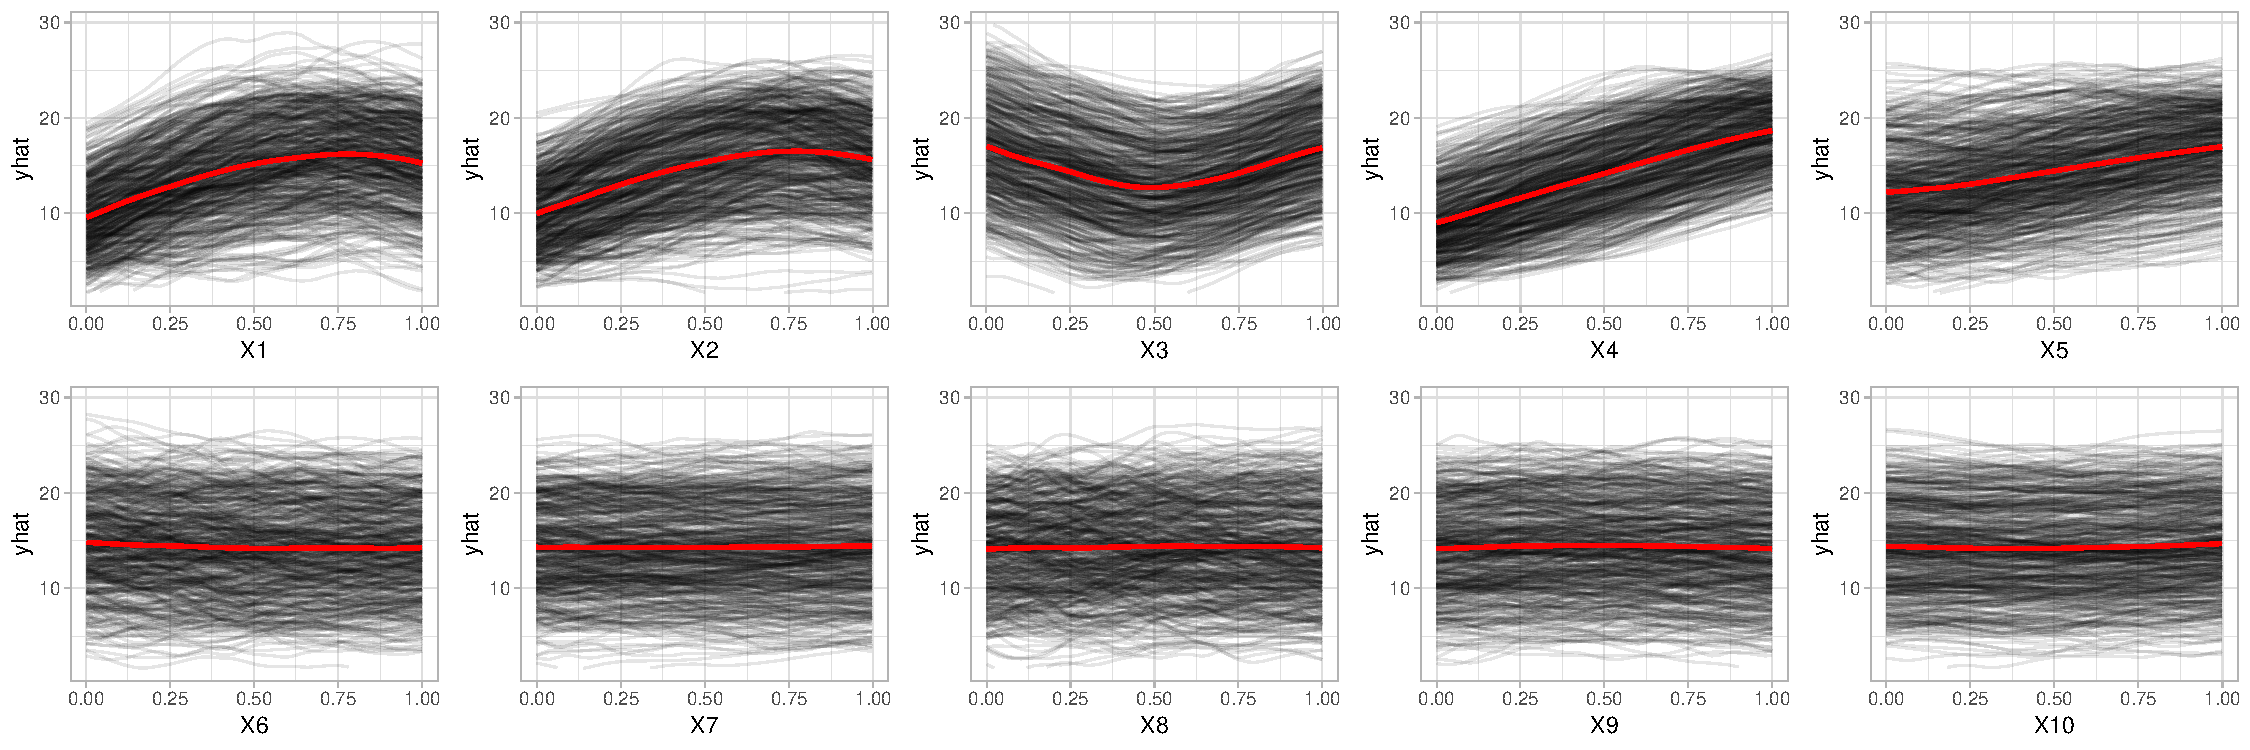
\includegraphics[width=1\linewidth]{figures/ice-ppr} 
  \caption{ICE curves for each feature in the PPR model fit to the simulated Friedman data. The red curve represents the PDP (i.e., the averaged ICE curves).}
  \label{fig:ice-ppr}
\end{figure}

Obtaining the ICE-based feature importance scores is also straightforward, just specify \code{method = "ice"} in the call to \code{vip::vi()} or \code{vip::vip()}. This is illustrated in the code chunk below and the results are Figure~\ref{fig:vip-ice-ppr-nn} are similar to those obtained using the PDP method.

\begin{example}
# Plot VI scores
p1 <- vip(pp, method = "ice") + ggtitle("PPR")
p2 <- vip(nn, method = "ice") + ggtitle("NN")

# Figure 9
grid.arrange(p1, p2, ncol = 2)
\end{example}

\begin{figure}[!htb]
  \centering 
  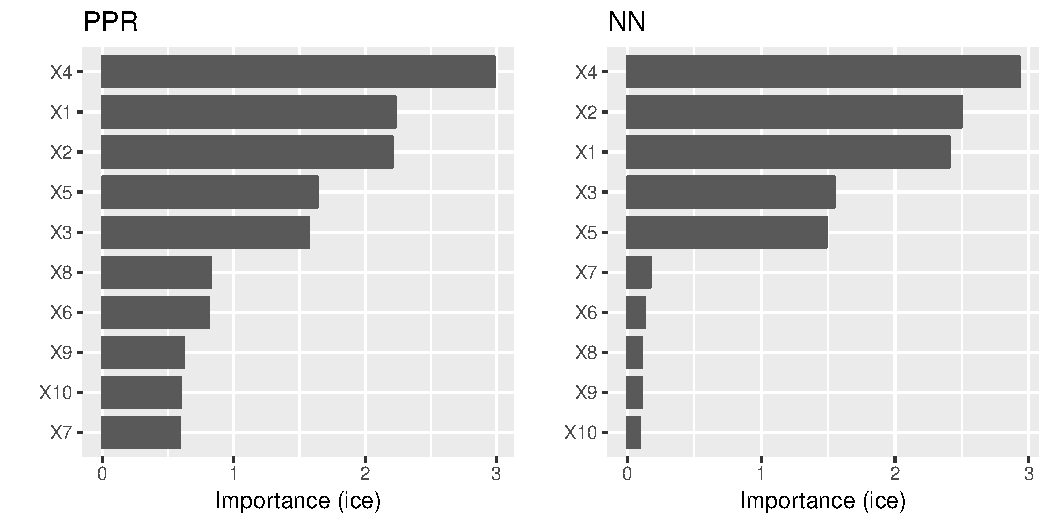
\includegraphics[width=1\linewidth]{figures/vip-ice-ppr-nn} 
  \caption{ICE-based feature importance for the PPR and NN models fit to the simulated Friedman data.}
  \label{fig:vip-ice-ppr-nn}
\end{figure}

When using \code{method = "pdp"} or \code{method = "ice"}, the feature effect values are stored as attributes \code{"pdp"} and \code{"ice"}, respectively. This is a convenience so that the feature effect plots (e.g., PDPs and ICE curves) can easily be reconstructed and compared with the VI scores, as demonstrated in the example below (see Figure~\ref{fig:pdp-from-attr}):

\begin{example}
# Construct PDP-based variable importance scores
vis <- vi(pp, method = "pdp")
#> Warning message:
#> Setting `method = "pdp"` is experimental, use at your own risk! 
vis
#> # A tibble: 10 x 2
#>    Variable Importance
#>    <chr>         <dbl>
#>  1 X4           2.93  
#>  2 X2           2.05  
#>  3 X1           2.04  
#>  4 X5           1.53  
#>  5 X3           1.38  
#>  6 X6           0.183 
#>  7 X10          0.139 
#>  8 X9           0.113 
#>  9 X8           0.0899
#> 10 X7           0.0558

# Reconstruct PDPs for all 10 features
par(mfrow = c(2, 5))
for (name in paste0("X", 1:10)) {
  plot(attr(vis, which = "pdp")[[name]], type = "l", ylim = c(9, 19), las = 1)
}
\end{example}

\begin{figure}[!htb]
  \centering 
  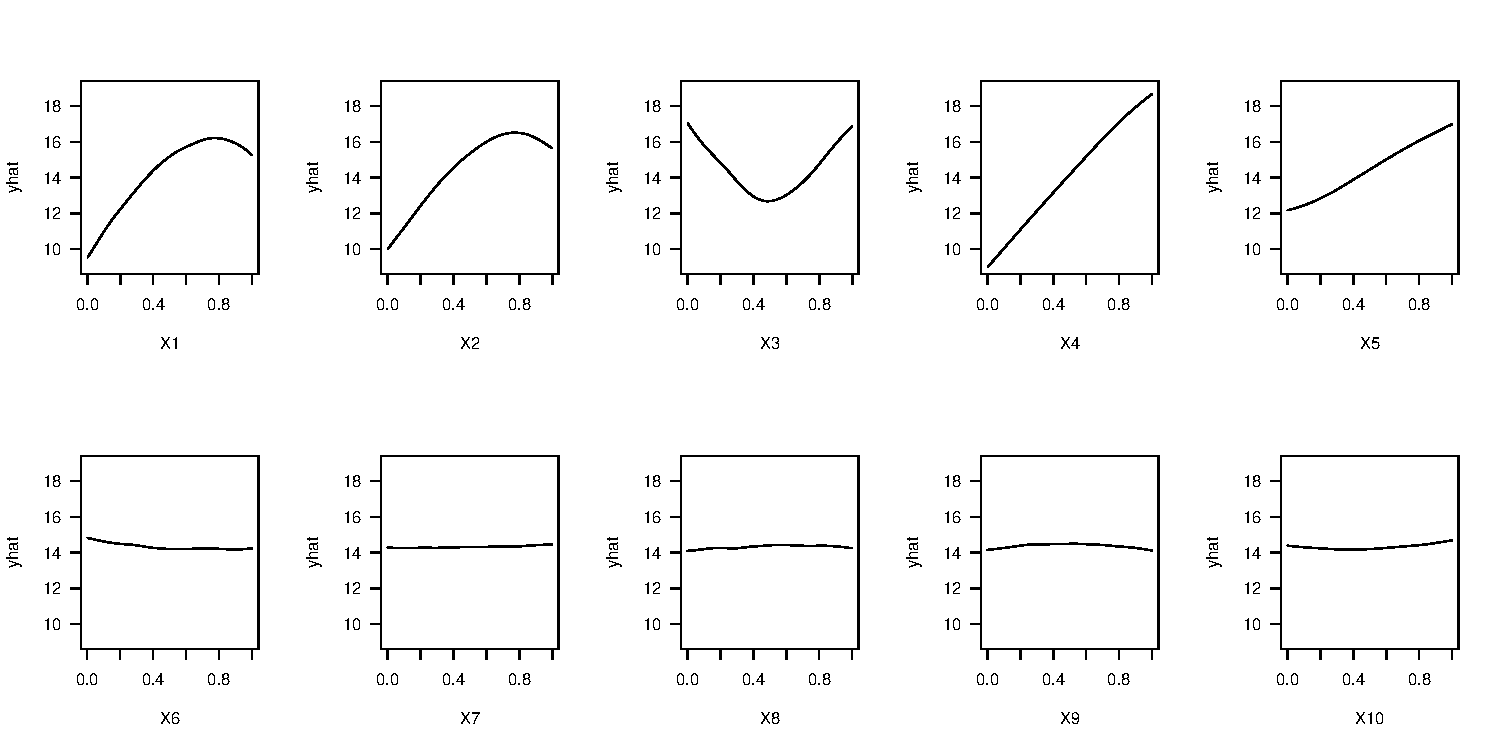
\includegraphics[width=1\linewidth]{figures/pdp-from-attr.pdf} 
  \caption{PDPs for all ten features reconstructed from the \code{"pdp"} attribute of the \code{vis} object.}
  \label{fig:pdp-from-attr}
\end{figure}

\subsection{Permutation method}

The permutation method exists in various forms and was made popular in \citet{random-breiman-2001} for RFs, before being generalized and extended in \citet{fisher-model-2018}. The permutation approach used in \pkg{vip} is quite simple and is outlined in Algorithm~\ref{alg:permute} below. The idea is that if we randomly permute the values of an important feature in the training data, the training performance would degrade (since permuting the values of a feature effectively destroys any relationship between that feature and the target variable). This of course assumes that the model has been properly tuned (e.g., using cross-validation) and is not over fitting. The permutation approach uses the difference between some baseline performance measure (e.g., training $R^2$, AUC, or RMSE) and the same performance measure obtained after permuting the values of a particular feature in the training data (\strong{Note:} the model is NOT refit to the training data after randomly permuting the values of a feature). It is also important to note that this method may not be appropriate when you have, for example, highly correlated features (since permuting one feature at a time may lead to unlikely data instances). 

Let $X_1, X_2, \dots, X_j$ be the features of interest and let $\mathcal{M}_{orig}$ be the baseline performance metric for the trained model; for brevity, we'll assume smaller is better (e.g., classification error or RMSE). The permutation-based importance scores can be computed as follows:

\begin{algorithm}
\begin{enumerate}
  \item For $i = 1, 2, \dots, j$:
  \begin{enumerate}
    \item Permute the values of feature $X_i$ in the training data.
    \item Recompute the performance metric on the permuted data $\mathcal{M}_{perm}$.
    \item Record the difference from baseline using $imp\left(X_i\right) = \mathcal{M}_{perm} - \mathcal{M}_{orig}$.
  \end{enumerate}
  \item Return the VI scores $imp\left(X_1\right), imp\left(X_2\right), \dots, imp\left(X_j\right)$.
\end{enumerate}
\caption{A simple algorithm for constructing permutation-based VI scores. \label{alg:permute}}
\end{algorithm}

Algorithm~\ref{alg:permute} can be improved or modified in a number of ways. For instance, the process can be repeated several times and the results averaged together. This helps to provide more stable VI scores, and also the opportunity to measure their variability. Rather than taking the difference in step (c), \citet[Chapter 5, Section 5.5.4]{molnar-2019-iml} argues that using the ratio $\mathcal{M}_{perm} / \mathcal{M}_{orig}$ makes the importance scores more comparable across different problems. It's also possible to assign importance scores to groups of features (e.g., by permuting more than one feature at a time); this would be useful if features can be categorized into mutually exclusive groups, for instance, categorical features that have been \dfn{one-hot-encoded}.

To use the permutation approach in \pkg{vip}, specify \code{method = "permute"} in the call to \code{vi()} or \code{vip()}. Note that using \code{method = "permute"} requires specifying a few additional arguments (e.g., the training data, target name, etc.); see \code{?vi\_permute} for details.

An example is given below for the previously fitted PPR and NN models. Here we use $R^2$ (\code{metric = "rsquared"}) as the evaluation metric. The results, which are displayed in Figure~\ref{fig:vip-permute-ppr-nn}, agree with those obtained using the PDP- and ICE-based methods.

\begin{example}
# Plot VI scores
set.seed(2021)  # for reproducibility
p1 <- vip(pp, method = "permute", target = "y", metric = "rsquared",
          pred_wrapper = predict) + ggtitle("PPR")
p2 <- vip(nn, method = "permute", target = "y", metric = "rsquared",
          pred_wrapper = predict) + ggtitle("NN")

# Figure 11
grid.arrange(p1, p2, ncol = 2)
\end{example}

\begin{figure}[!htb]
  \centering 
  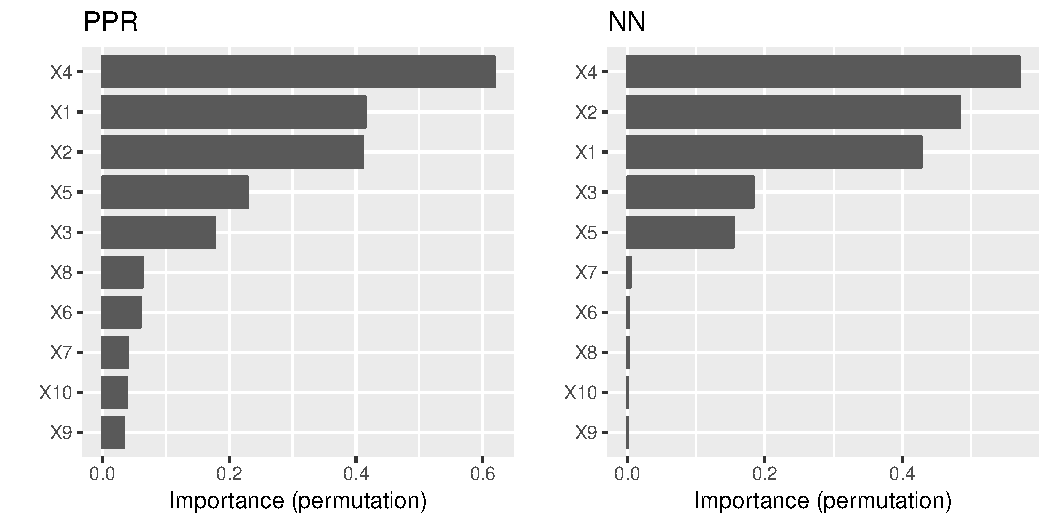
\includegraphics[width=1\linewidth]{figures/vip-permute-ppr-nn} 
  \caption{Permutation-based feature importance for the PPR and NN models fit to the simulated Friedman data.}
  \label{fig:vip-permute-ppr-nn}
\end{figure}

The permutation approach introduces randomness into the procedure and therefore should be run more than once if computationally feasible. Fortunately, this also allows us to compute standard errors for the estimated VI scores, as illustrated in the example below where we specify \code{nsim = 10} to request that each feature be permuted 10 times and the results averaged together.

\begin{example}
# Use 10 Monte Carlo reps
set.seed(403)  # for reproducibility
vi(pp, method = "permute", target = "y", metric = "rsquared",
   pred_wrapper = predict, nsim = 10)

# A tibble: 10 x 3
#>    Variable Importance   StDev
#>    <chr>         <dbl>   <dbl>
#>  1 X4           0.586  0.0188 
#>  2 X2           0.416  0.0184 
#>  3 X1           0.377  0.0162 
#>  4 X5           0.222  0.0155 
#>  5 X3           0.183  0.00936
#>  6 X6           0.0620 0.00379
#>  7 X8           0.0603 0.00378
#>  8 X9           0.0389 0.00417
#>  9 X7           0.0373 0.00321
#> 10 X10          0.0348 0.00290
\end{example}

All available performance metrics for regression and classification can be listed using the \code{list\_metrics()} function, for example:

\begin{example}
#>     Metric                       Description                      Task
#> 1      auc            Area under (ROC) curve     Binary classification
#> 2    error           Misclassification error     Binary classification
#> 3  logloss                          Log loss     Binary classification
#> 4     mauc Multiclass area under (ROC) curve Multiclass classification
#> 5 mlogloss               Multiclass log loss Multiclass classification
#> 6      mse                Mean squared error                Regression
#> 7       r2                         R squared                Regression
#> 8 rsquared                         R squared                Regression
#> 9     rmse           Root mean squared error                Regression
\end{example}

We can also use a custom metric (i.e., loss function). Suppose for example you want to measure importance using the \dfn{mean absolute error} (MAE): 

\begin{equation}
  MAE = \frac{1}{n}\sum_{i = 1}^n\left|Y_i - \widehat{f}\left(\boldsymbol{X}_i\right)\right|,
\end{equation}

where $\widehat{f}\left(\boldsymbol{X}_i\right)$ is the predicted value of $Y_i$. A simple function implementing this metric is given below (note that, according to the documentation in \code{?vi\_permute}, this function requires two arguments: \code{actual} and \code{predicted}).

\begin{example}
mae <- function(actual, predicted) {
  mean(abs(actual - predicted))
}
\end{example}

To use this for computing permutation-based VI scores just pass it via the \code{metric} argument (be warned, however, that the metric used for computing permutation importance should be the same as the metric used to train and tune the model). Also, since this is a custom metric, we need to specify whether a smaller value indicates better performance by setting \code{smaller\_is\_better = TRUE}. The results, which are displayed in Figure~\ref{fig:vip-nn-mae}, are similar to those in Figure~\ref{fig:vip-permute-ppr-nn}, albeit a different scale. 

\begin{example}
# Figure 12
set.seed(2321)  # for reproducibility
vip(nn, method = "permute", target = "y", metric = mae,
    smaller_is_better = TRUE, pred_wrapper = nnet:::predict.nnet) +
  ggtitle("Custom loss function: MAE")
\end{example}

\begin{figure}[!htb]
  \centering
  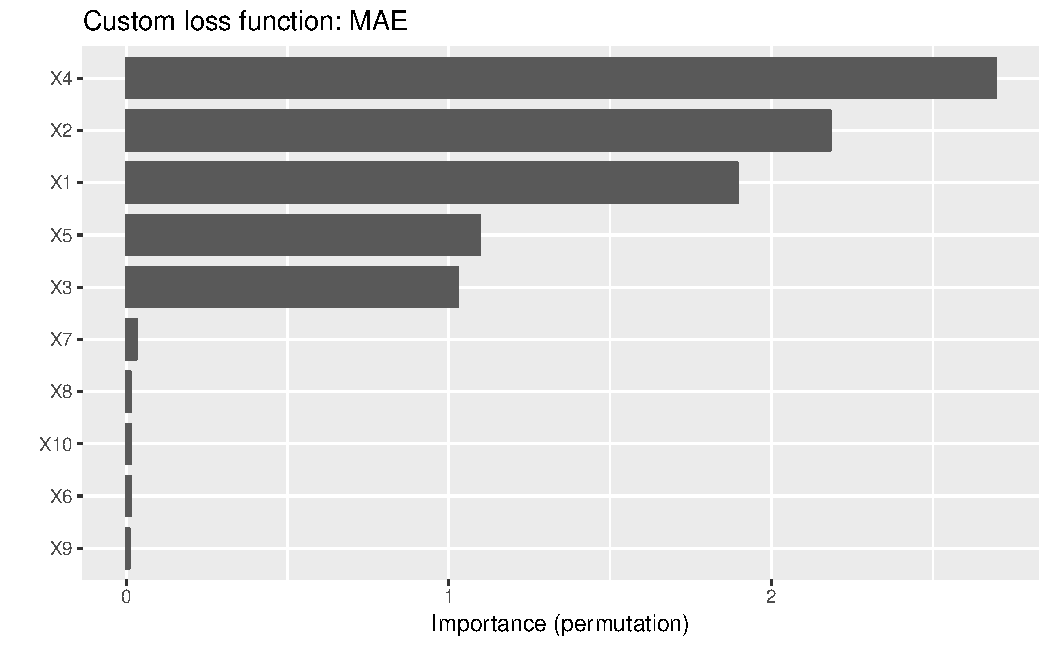
\includegraphics[width=1\linewidth]{figures/vip-permute-nn-mae}
  \caption{Permutation-based feature importance for the NN model fit to the simulated Friedman data. In this example, permutation importance is based on the MAE metric.}
  \label{fig:vip-nn-mae}
\end{figure}

Although permutation importance is most naturally computed on the training data, it may also be useful to do the shuffling and measure performance on new data! This is discussed in depth in \citet{molnar-2019-iml}[Chapter 5, Section 5.2]. For users interested in computing permutation importance using new data, just supply it to the \code{train} argument in the call to \code{vi()}, \code{vip()}, or \code{vi\_permute()}. For instance, suppose we wanted to only use a fraction of the original training data to carry out the computations. In this case, we could simply pass the sampled data to the \code{train} argument as follows:

\begin{example}
# Figure 13
set.seed(2327)  # for reproducibility
vip(nn, method = "permute", 
    train = trn[sample(nrow(trn), size = 400), ],  # sample 400 observations
    target = "y", metric = "rmse") +
  ggtitle("Using a random subset of training data")
\end{example}

\begin{figure}[!htb]
  \centering
  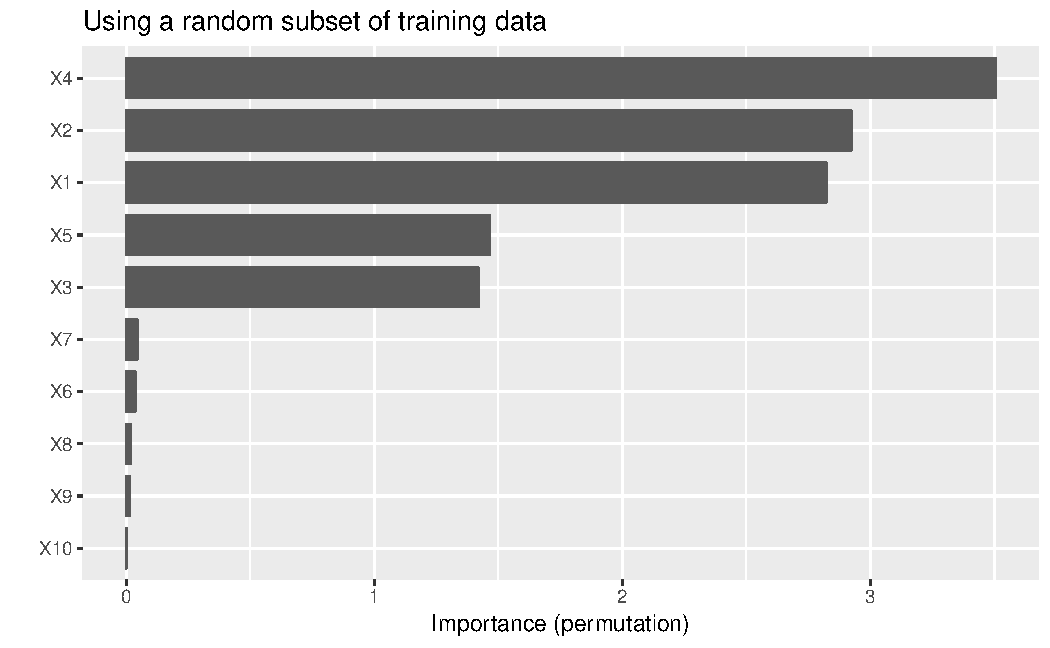
\includegraphics[width=1\linewidth]{figures/vip-permute-nn-sample}
  \caption{Permutation-based feature importance for the NN model fit to the simulated Friedman data. In this example, permutation importance is based on a random sample of 400 training observations.}
  \label{fig:vip-nn-mae}
\end{figure}

When using the permutation method with \code{nsim > 1}, the default is to keep all the permutation scores as an attribute called \code{"raw\_scores"}; you can turn this behavior off by setting \code{keep = FALSE} in the call to \code{vi\_permute()}, \code{vi()}, or \code{vip()}. If \code{keep = TRUE} and \code{nsim > 1}, you can request all permutation scores to be plotted by setting \code{all\_permutation = TRUE} in the call to \code{vip()} as demonstrated in the code chunk below (see Figure~\ref{fig:vip-nn-mae}). This let's you visually inspect the variability in the permutation scores within each feature.

\begin{example}
# Figure 14
set.seed(8264)  # for reproducibility
vip(nn, method = "permute", target = "y", metric = "rmse",
    all_permutations = TRUE) +
  ggtitle("Plotting all permutation scores")
\end{example}

\begin{figure}[!htb]
  \centering
  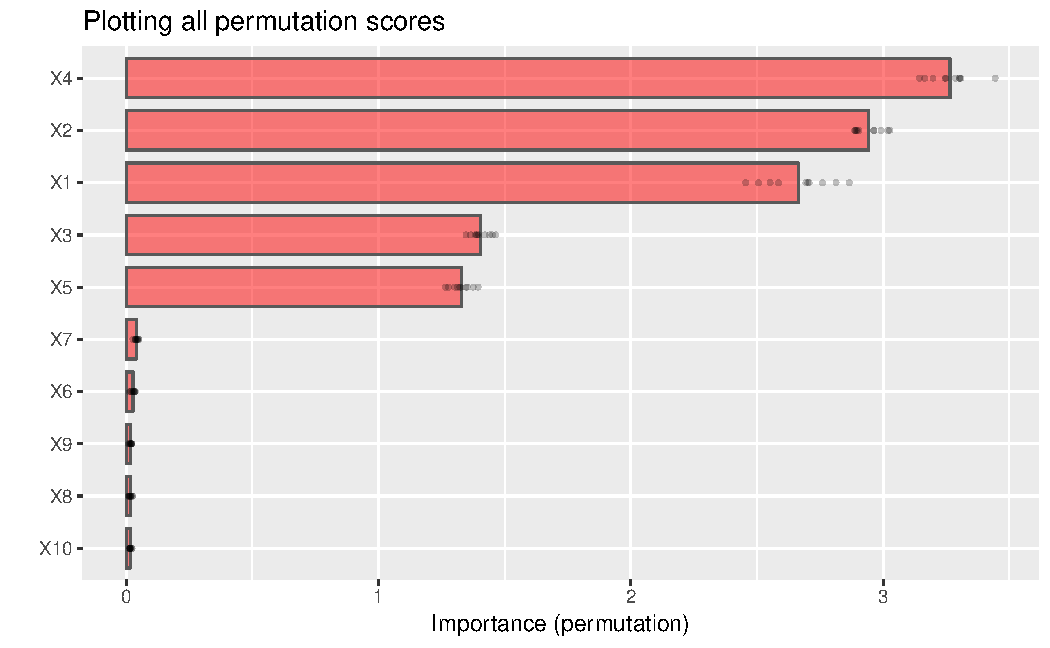
\includegraphics[width=1\linewidth]{figures/vip-permute-nn-all}
  \caption{Permutation-based feature importance for the NN model fit to the simulated Friedman data. In this example, all the permutation importance scores (points) are displayed for each feature along with their average (bars).}
  \label{fig:vip-permute-nn-all}
\end{figure}


% ------------------------------------------------------------------------------
\subsection{Benchmarks}
% ------------------------------------------------------------------------------

In this section, we compare the performance of three implementations of permutation-based VI scores: \code{iml::FeatureImp()}, \code{ingredients::feature\_importance()}, and \code{vip::vi()}.

We simulated 10,000 training observations from the Friedman 1 benchmark problem and trained a random forest using the \pkg{ranger} package. For each implementation, we computed permutation-based VI scores 100 times using the \CRANpkg{microbenchmark} package \citep{microbenchmark-pkg}. For this benchmark we did not use any of the parallel processing capability available in the \pkg{iml} and \pkg{vip} implementations. The results from \pkg{microbenchmark} are displayed in Figure~\ref{fig:benchmark} and summarized in the output below. In this case, the \pkg{vip} package was the most efficient, followed closely by \pkg{ingredients}. It should be noted, however, that the implementations in \pkg{vip} and \pkg{iml} can be parallelized. To the best of our knowledge, this is not the case for \pkg{ingredients}.

\begin{example}
Unit: seconds
        expr       min        lq      mean    median        uq      max neval cld
 ingredients  4.960832  5.658127  8.103375  5.853441  8.034572 61.61415   100  b 
         iml 10.636616 11.742197 14.760306 12.180391 12.961056 35.28671   100   c
         vip  4.076012  4.729765  5.968943  4.838916  5.745905 20.04089   100 a
\end{example}

\begin{figure}[!htb]
  \centering
  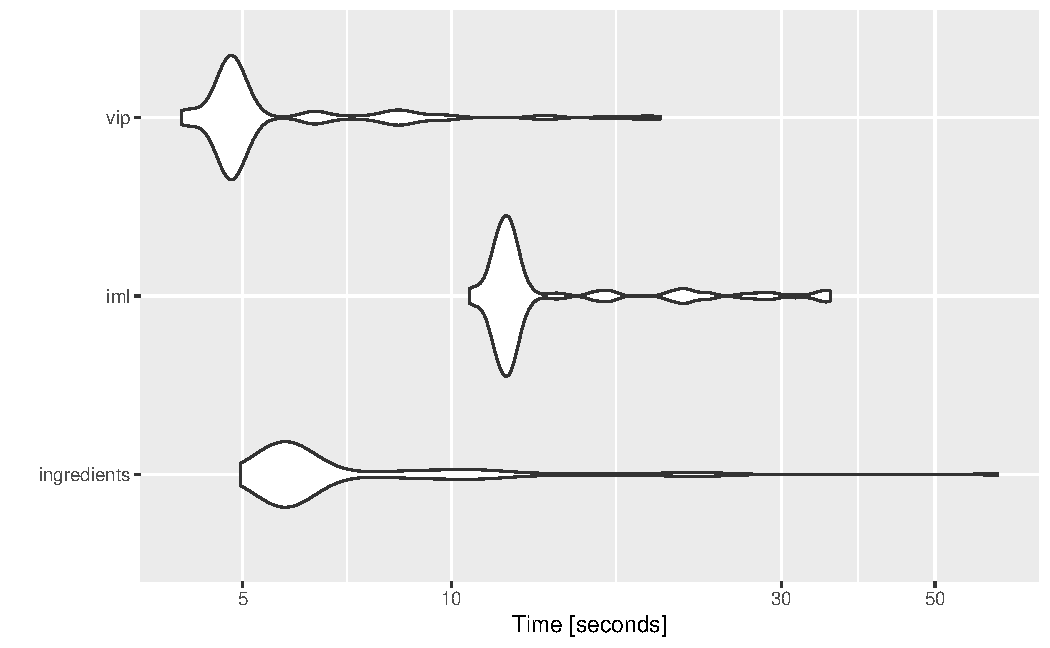
\includegraphics[width=1\linewidth]{figures/benchmark}
  \caption{Violin plots comparing the computation time from three different implementations of permutation-based VI scores across 100 simulations.}
  \label{fig:vip-permute-nn-all}
\end{figure}


% ------------------------------------------------------------------------------
\section{Use sparklines to characterize feature effects}
% ------------------------------------------------------------------------------

Starting with \pkg{vip} 0.1.3, we have included a new function \code{add\_sparklines()} for constructing HTML-based VI tables; however, this feature requires the \CRANpkg{DT} package \citep{DT-pkg}. The primary difference between \code{vi()} and \code{add\_sparklines()} is that the latter includes an \code{Effect} column that displays a sparkline representation of the partial dependence function for each feature. This is a concise way to display both feature importance and feature effect information in a single (interactive) table. See \code{?vip::add\_sparklines} for details. We illustrate the basic use of \code{add\_sparklines()} in the code chunks below.

\begin{example}
# First, compute a tibble of variable importance scores using any method
var_imp <- vi(rfo, method = "permute", metric = "rmse", target = "y")

# Next, convert to an html-based data table with sparklines
add_sparklines(var_imp, fit = rfo)
\end{example}

\begin{figure}[!htb]
  \centering 
  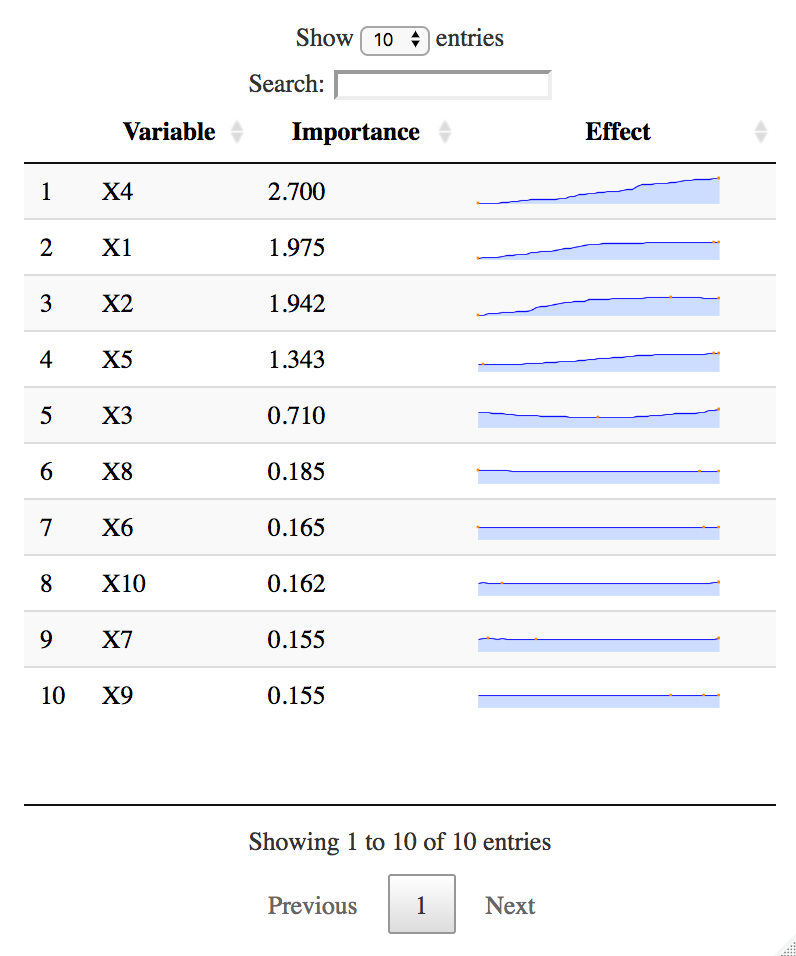
\includegraphics[width=1\linewidth]{figures/sparklines} 
  \caption{VIP with sparkline representation of feature effects fit to the simulated Friedman data.}
  \label{fig:sparklines}
\end{figure}


% ------------------------------------------------------------------------------
\section{Ames housing example}
% ------------------------------------------------------------------------------

For illustration, we'll use the Ames housing data which are available in the \CRANpkg{AmesHousing} package \citep{AmesHousing-pkg}. These data describe the sale of individual residential properties in Ames, Iowa from 2006--2010. The data set contains 2930 observations, 80 features (23 nominal, 23 ordinal, 14 discrete, and 20 continuous), and a continuous target giving the sale price of the home. The version we'll load is a cleaned up version of the original data set and treats all categorical variables as nominal (see \code{?AmesHousing::make\_ames} for details).

Using the R package \CRANpkg{SuperLearner} \citep{SuperLearner-pkg}, we trained five models using 5-fold cross-validation: a GBM using the \CRANpkg{xgboost} package \citep{xgboost-pkg}, an RF using the \CRANpkg{ranger} package \citep{ranger-pkg}, a MARS model using the \pkg{earth} package, a GLMNET model using the \CRANpkg{glmnet} package \citep{glmnet-pkg}, and a support vector regression model using the \CRANpkg{kernlab} package \citep{kernlab-pkg}. The coefficients from the meta learner indicate that the GBM contributes the most to new predictions, followed by the MARS model, RF, and the GLMNET. The support vector regression model did not contribute to the ensemble.

\begin{example}
# Load the Ames housing data
ames <- AmesHousing::make_ames()
X <- subset(ames, select = -Sale_Price)
y <- ames$Sale_Price

# Load required packages
library(SuperLearner)

# List of base learners
learners <- c("SL.xgboost", "SL.ranger", "SL.earth", "SL.glmnet", "SL.ksvm")

# Stack models
set.seed(840)
ctrl <- SuperLearner.CV.control(V = 5L, shuffle = TRUE)
sl <- SuperLearner(Y = y, X = X, SL.library = learners, verbose = TRUE,
                   cvControl = ctrl)
sl
#>  Call:  
#> SuperLearner(Y = y, X = X, SL.library = learners, verbose = TRUE,  
#>     cvControl = ctrl) 
#> 
#> 
#>                      Risk        Coef
#> SL.xgboost_All  527111540 0.603160823
#> SL.ranger_All   658707534 0.111650583
#> SL.earth_All    731657510 0.276895806
#> SL.glmnet_All   884821443 0.008292788
#> SL.ksvm_All    6782709110 0.000000000
\end{example}

In the code chunks below we request permutation-based VI scores and add sparkline representations of the PDPs for the top ten features. For this we need to define a couple of wrapper functions. One for computing predictions (for the permutation VI scores) and one for computing averaged predictions (for the PDPs):

\begin{example}
# Prediction wrapper functions
imp_fun <- function(object, newdata) {  # for permutation-based VI scores
  predict(object, newdata = newdata)$pred
}
par_fun <- function(object, newdata) {  # for PDPs
  mean(predict(object, newdata = newdata)$pred)
}
\end{example}

To speed up the process, we perform the computations in parallel by setting \code{parallel = TRUE} in the call to \code{vi()} and \code{add\_sparklines()}. Note that we first need to set up a parallel backend for this to work. Both \pkg{vip} and \pkg{pdp} use \CRANpkg{plyr} \citep{plyr-pkg}---which relies on \CRANpkg{foreach} \citep{foreach-pkg}---so any parallel backend supported by the \pkg{foreach} package should work. Below we use a \dfn{socket} approach with the \CRANpkg{doParallel} backend \citep{doParallel-pkg} using a cluster of size five.

\begin{example}
# Setup parallel backend
library(doParallel) # load the parallel backend
cl <- makeCluster(5) # use 5 workers
registerDoParallel(cl) # register the parallel backend

# Permutation-based feature importance
set.seed(278)
var_imp <- vi(sl, method = "permute", train = X, target = y, metric = "rmse",
              pred_wrapper = imp_fun, nsim = 5, parallel = TRUE)

# Add sparkline representation of feature effects
add_sparklines(var_imp[1L:10L, ], fit = sl, pred.fun = par_fun, train = X, 
               digits = 2, verbose = TRUE, trim.outliers = TRUE, 
               grid.resolution = 20, parallel = TRUE)
               
# Shut down cluster
stopCluster(cl)
\end{example}

\begin{figure}[!htb]
  \centering 
  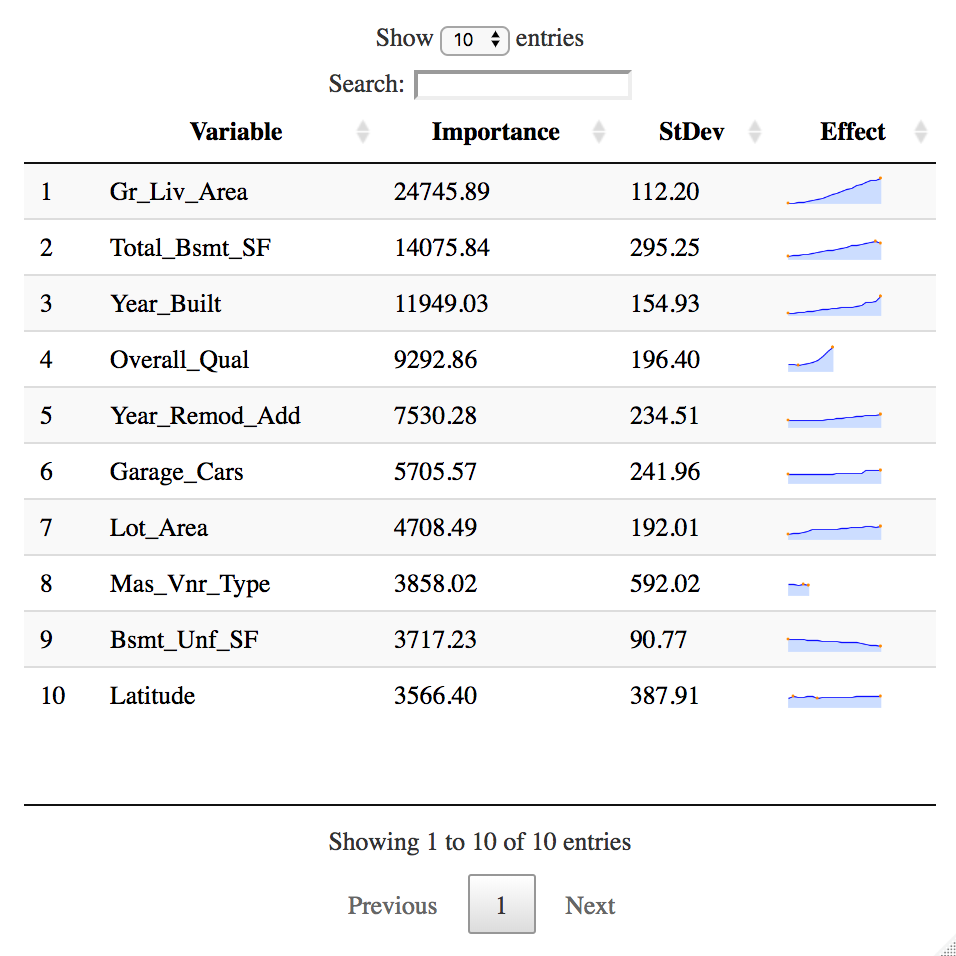
\includegraphics[width=1\linewidth]{figures/ames-sparklines} 
  \caption{VIP with sparkline representation of feature effects for the top ten features from a Super Learner fit to the Ames housing data.}
  \label{fig:sparklines}
\end{figure}


% ------------------------------------------------------------------------------
\section{Summary}
% ------------------------------------------------------------------------------

VIPs help to visualize the strength of the relationship between each feature and the response, while accounting for all the other features in the model. We've discussed two types of VI: model-specific and model-agnostic, as well as some of their strengths and weaknesses. In this paper, we showed how to construct VIPs for various types of "black box" models in R using the \pkg{vip} package. We also briefly discussed related approaches available in other R packages. Suggestions to avoid high execution times were discussed and demonstrated via examples. This paper is based on \pkg{vip} version 0.1.3. For updates that have occurred since then, see the package’s \href{https://cran.r-project.org/web/packages/vip/news/news.html}{NEWS file}. In terms of future development, \pkg{vip} can be expanded in a number of ways. For example, we plan to incorporate the option to compute group-based permutation scores. We're also working on including a new option for efficiently computing Shapley-based VI scores via the new \href{https://github.com/bgreenwell/fastshap}{fastshap} package. Although not discussed in this paper, the package also includes a promising statistic (similar to the PDP- and ICE-based VI scores previously discussed) for measuring the relative strength of interaction between features. 


% ------------------------------------------------------------------------------
\section{Acknowledgments}
% ------------------------------------------------------------------------------

TBD.


\bibliography{greenwell-boehmke}

\address{Brandon M. Greenwell\\
  University of Cincinnati\\
  2925 Campus Green Dr\\
  Cincinnati, OH 45221\\
  United States of America\\
  ORCiD: \href{https://orcid.org/0000-0002-8120-0084}{0000-0002-8120-0084}\\
  \email{greenwell.brandon@gmail.com}}

\address{Bradley C. Boehmke\\
  University of Cincinnati\\
  2925 Campus Green Dr\\
  Cincinnati, OH 45221\\
  United States of America\\
  ORCiD: \href{https://orcid.org/0000-0002-3611-8516}{0000-0002-3611-8516}\\
  \email{bradleyboehmke@gmail.com}}
